NOTE: This text is about the model in examples/diffserv/onedomain, which could be turned into a showcase.

\subsection{One domain example}

The \ffilename{examples/diffserv/onedomain} directory contains
a network in which the routers constitute a single DiffServ domain.
Several experiments are performed on this network, that demonstrates
the resource allocation, and flow isolation capabilities of DiffServ
network compared to the Best Effort service. It also shows the
behavior of the different forwarding classes. These experiments
reproduce the results obtained by an NS3 DiffServ implementation
(\cite{Sanjay2010}).

The network composed of 8 hosts and 6 routers.
Hosts are connected to the routers by 100Mbps Ethernet links. The
routers are connected by PPP lines with lower datarates.
Traffic policing performed at the Ethernet interface of the edge
routers (\ttt{R0},\ttt{R1},\ttt{R4},\ttt{R5}). By changing
the queue module of the PPP interfaces, diverse per-hop behaviors
can be instrumented.

\begin{center}
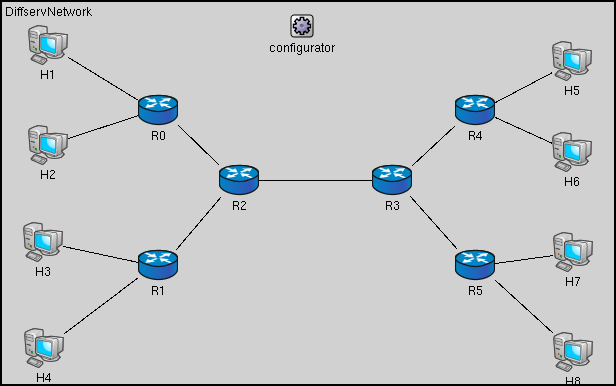
\includegraphics[scale=0.5]{figures/OneDomainDiffservNetwork.png}
\end{center}

Traffic flows from hosts \ttt{H1-H4} to hosts \ttt{H5-H8}. The source hosts
configured to send voice and video data to the destinations hosts. The voice
is sent by an \nedtype{UDPBacisBurst} application, with mean burst duration
352ms, and mean sleep duration 650ms; this mirrors the talk/listen phases
of a phone call. 172 bytes long packets (160 byte data + 12 byte RTP header)
are sent in every 20ms in the burst phase. Considering the IP+UDP overhead,
this results a 80kbps peek rate, and approximately 28kbps avarege rate for
the voice traffic. The video streaming application is modeled by a ~100kbps
CBR traffic, 500 bytes are sent in every 40ms by an \nedtype{UDPBasicApp}
application.

Traffic policing performed at the Ethernet interfaces of the edge routers
(\ttt{R0},\ttt{R1},\ttt{R4},\ttt{R5}). For this purpose a traffic conditioner
is added to the ingress data path of the Ethernet interfaces. The necessary
forwarding behaviours are implemented by changing the external queue module
of the PPP interfaces of routers.

The following sections describe four experiments in detail. The experiments
are numbered from 1 to 5, but 4 is omitted, to keep it consistent with the
numbering in \cite{Sanjay2010}.
The ini file define the configurations for each experiment. Configurations
named \ttt{ExpXY} (where X and Y are digits) belong to Experiment X.
After running each configuration, result can be evaluated by executing
the \ffilename{ExperimentX.R} file with the
\href{http://www.r-project.org}{R statistical program}.

\subsubsection*{Experiment 1}

This experiment shows how the resources of a network can be allocated
to different forwarding classes, and also demontrates the effect of
these allocation on the quality of the service.

In configurations \ttt{Exp11-Exp15}, the traffic from hosts \ttt{H1-H4}
are marked with different AFx1 classes at the edge routers. These
forwarding classes are implemented by PPP queues using a WRR scheduler.
The weights of the different forwarding classes are changed from the most
polarized 7/6/5/4 to the least polarized 1/1/1/1. In the \ttt{Exp16}
configuration, packets of the \ttt{H4} host are classified as EF, so
they have higher priority at forwarding. The last configuration
(\ttt{Exp17}), describing a Best Effort network, serves as a reference
point for other measurements.

Results shows that packets that belong to different AFxy forwarding classes get
different treatments, and the differences are larger when the variance
of the weights is larger. It also can be observed that EF packets
receives much better treatment than others: they have no packet loss,
and have a very low delay.

\subsubsection*{Experiment 2}

This experiment shows how the different drop precedencies of the AFxy
forwarding classes can be implemented by RED queueing. In configurations
\ttt{Exp21-Exp24}, hosts \ttt{H1-H3} sends the normal voice and video
traffic, while \ttt{H4} sends only CBR traffic whose rate changes
from 10kbps to 100kpbs in 10kpbs (so there is 10 measurement for each
configuration). Packets from \ttt{H1-H3} are marked with
increasing drop priority (i.e. \ttt{H1} traffic is forwarded as AF11,
\ttt{H2} as AF12, and \ttt{H3} as AF13). The forwarding treatment
of \ttt{H4} traffic is changing in the different
configurations: AF11 in \ttt{Exp21}, AF12 in \ttt{Exp22}, and
AF13 in \ttt{Exp23}. The \ttt{Exp24} configuration shows the behavior
of a Best Effort network under the same traffic.

The plots shows that in the DiffServ network, there is no loss of
AF11 traffic, and AF12 traffic loss is very low. The average queue
length is lower in \ttt{Exp23}, because the red packets are dropped
more likely.

\subsubsection*{Experiment 3}

This experiment tests bandwidth utilization and flow isolation.
Only hosts \ttt{H1} and \ttt{H2} generate traffic. \ttt{H1} has
an extra \nedtype{UDPBasicApp} application, that generates a CBR
traffic in addition to the voice and video streams. The rate of
this extra traffic varies from 10kbps to 50kbps in 10kpbs steps
in different measurements. Because the PPP links have only
300kbps datarate, the link between \ttt{R2} and \ttt{R3} is
congested when the extra traffic is high enough.

With the first configuration (\ttt{Exp31}), both traffic policing
and DiffServ queues are used. Traffic is metered at the egde routers
by a token bucket meter. Packets whose rate is below 150kbps
marked as AF11, the excess traffic is marked as AF12. RED queues
in the network are configured so, that AF12 packets are dropped
more aggressively than AF11 packets.

With the second configuration (\ttt{Exp32}), only traffic policing
is used. Packets whose rate exceeding the allowed 150kbps limit
are dropped at the boundary of the domain. There is no differentiated
forwarding treatment of packets inside the domain. Each packet goes
to the same queue in the PPP interfaces of routers. They are simple
drop tail queues with 200 frames capacity.

The third configuration describes a Best Effort network.
There is not traffic policing, and the PPP interfaces contain
drop tail queues having buffer space for 200 frames.

As it is expected, the bandwith utilization is high in the first
and third case, but lower in the second case. On the other hand,
the Best Effort network does not provide the same flow isolation
as the DiffServ network. In the third case the well-behaving
\ttt{H3} node suffers from the extra traffic generated by \ttt{H1}.

\subsubsection*{Experiment 5}

This experiment compares a DiffServ network and a Best Effort network.
In the DiffServ network, all voice traffic is marked with EF class
at the edge routers. The video traffic originating from \ttt{H1} and
\ttt{H3} are marked with AF11, while video traffic from \ttt{H2} and
\ttt{H4} are marked with AF21. Routers contain DiffServQueue that
implements the EF and AFxy forwarding classes with priority queueing,
and weighted round-robin queueing. The weight of AF11 is a bit larger,
than the weight of AF21, so hosts \ttt{H1} and \ttt{H3} gets better
services. The queues contain a 100 frame buffer capacity for each forwarding
class.

In the Best Effort network each PPP queue is a \nedtype{DropTailQueue}.
The queue capacities are 200 frames, to keep the buffer space equal to
the DiffServ case.

In the DiffServ network, there is no loss of voice packets. Losses
of video packets are smaller for \ttt{H1} and \ttt{H3} hosts, and
higher for \ttt{H2} and \ttt{H4} than in a Best Effort network.
This is expected, because DiffServ cannot increase the available
resources, it only distributes them differently. It can also be
observed, that the delay of voice packets are much smaller in the
DiffServ network, so it can provide the necessary services for
VoIP applications, while a Best Effort network can not.

\subsection*{Multiple domains example}

This example describes a real-world scenario, and shows how
the SLAs can be implemented with the components offered by INET.
